\section{Lights, shadows and surface detail}
\label{sec:lights}
\begin{figure}[H]\centering
\begin{minipage}{0.49\linewidth}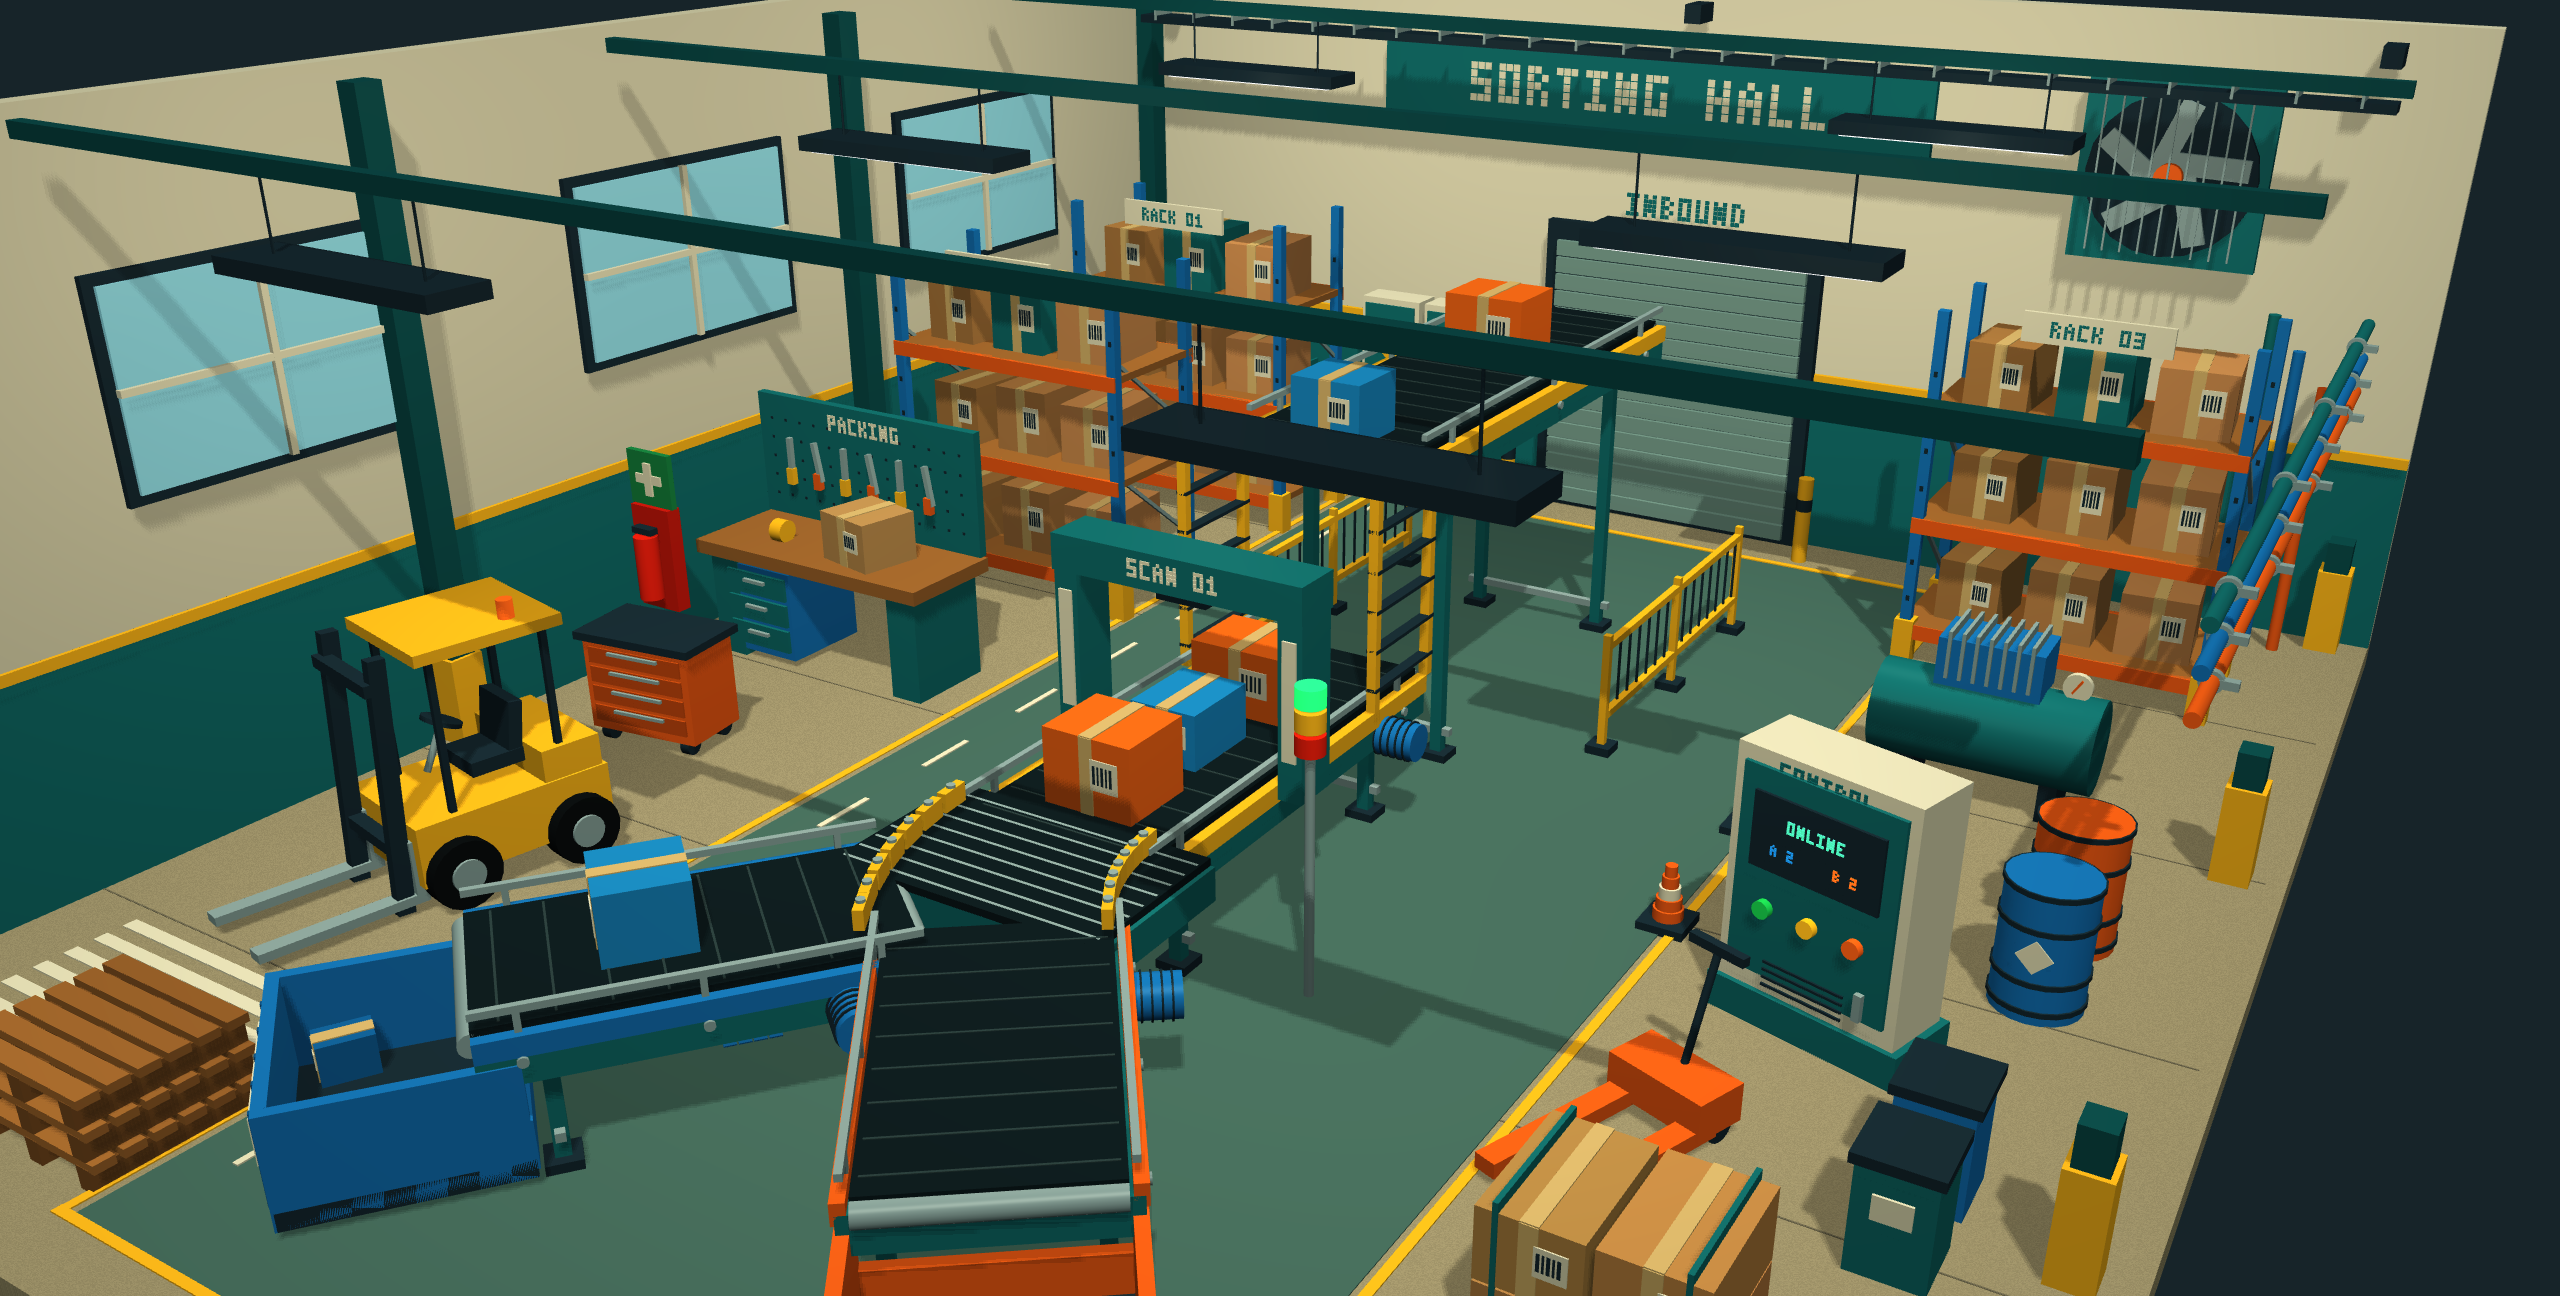
\includegraphics[width=\linewidth]{assets/lights_on_crop.png}\par\small\textbf{A. Point lights on:} warmer, brighter surfaces.\end{minipage}\hfill
\begin{minipage}{0.49\linewidth}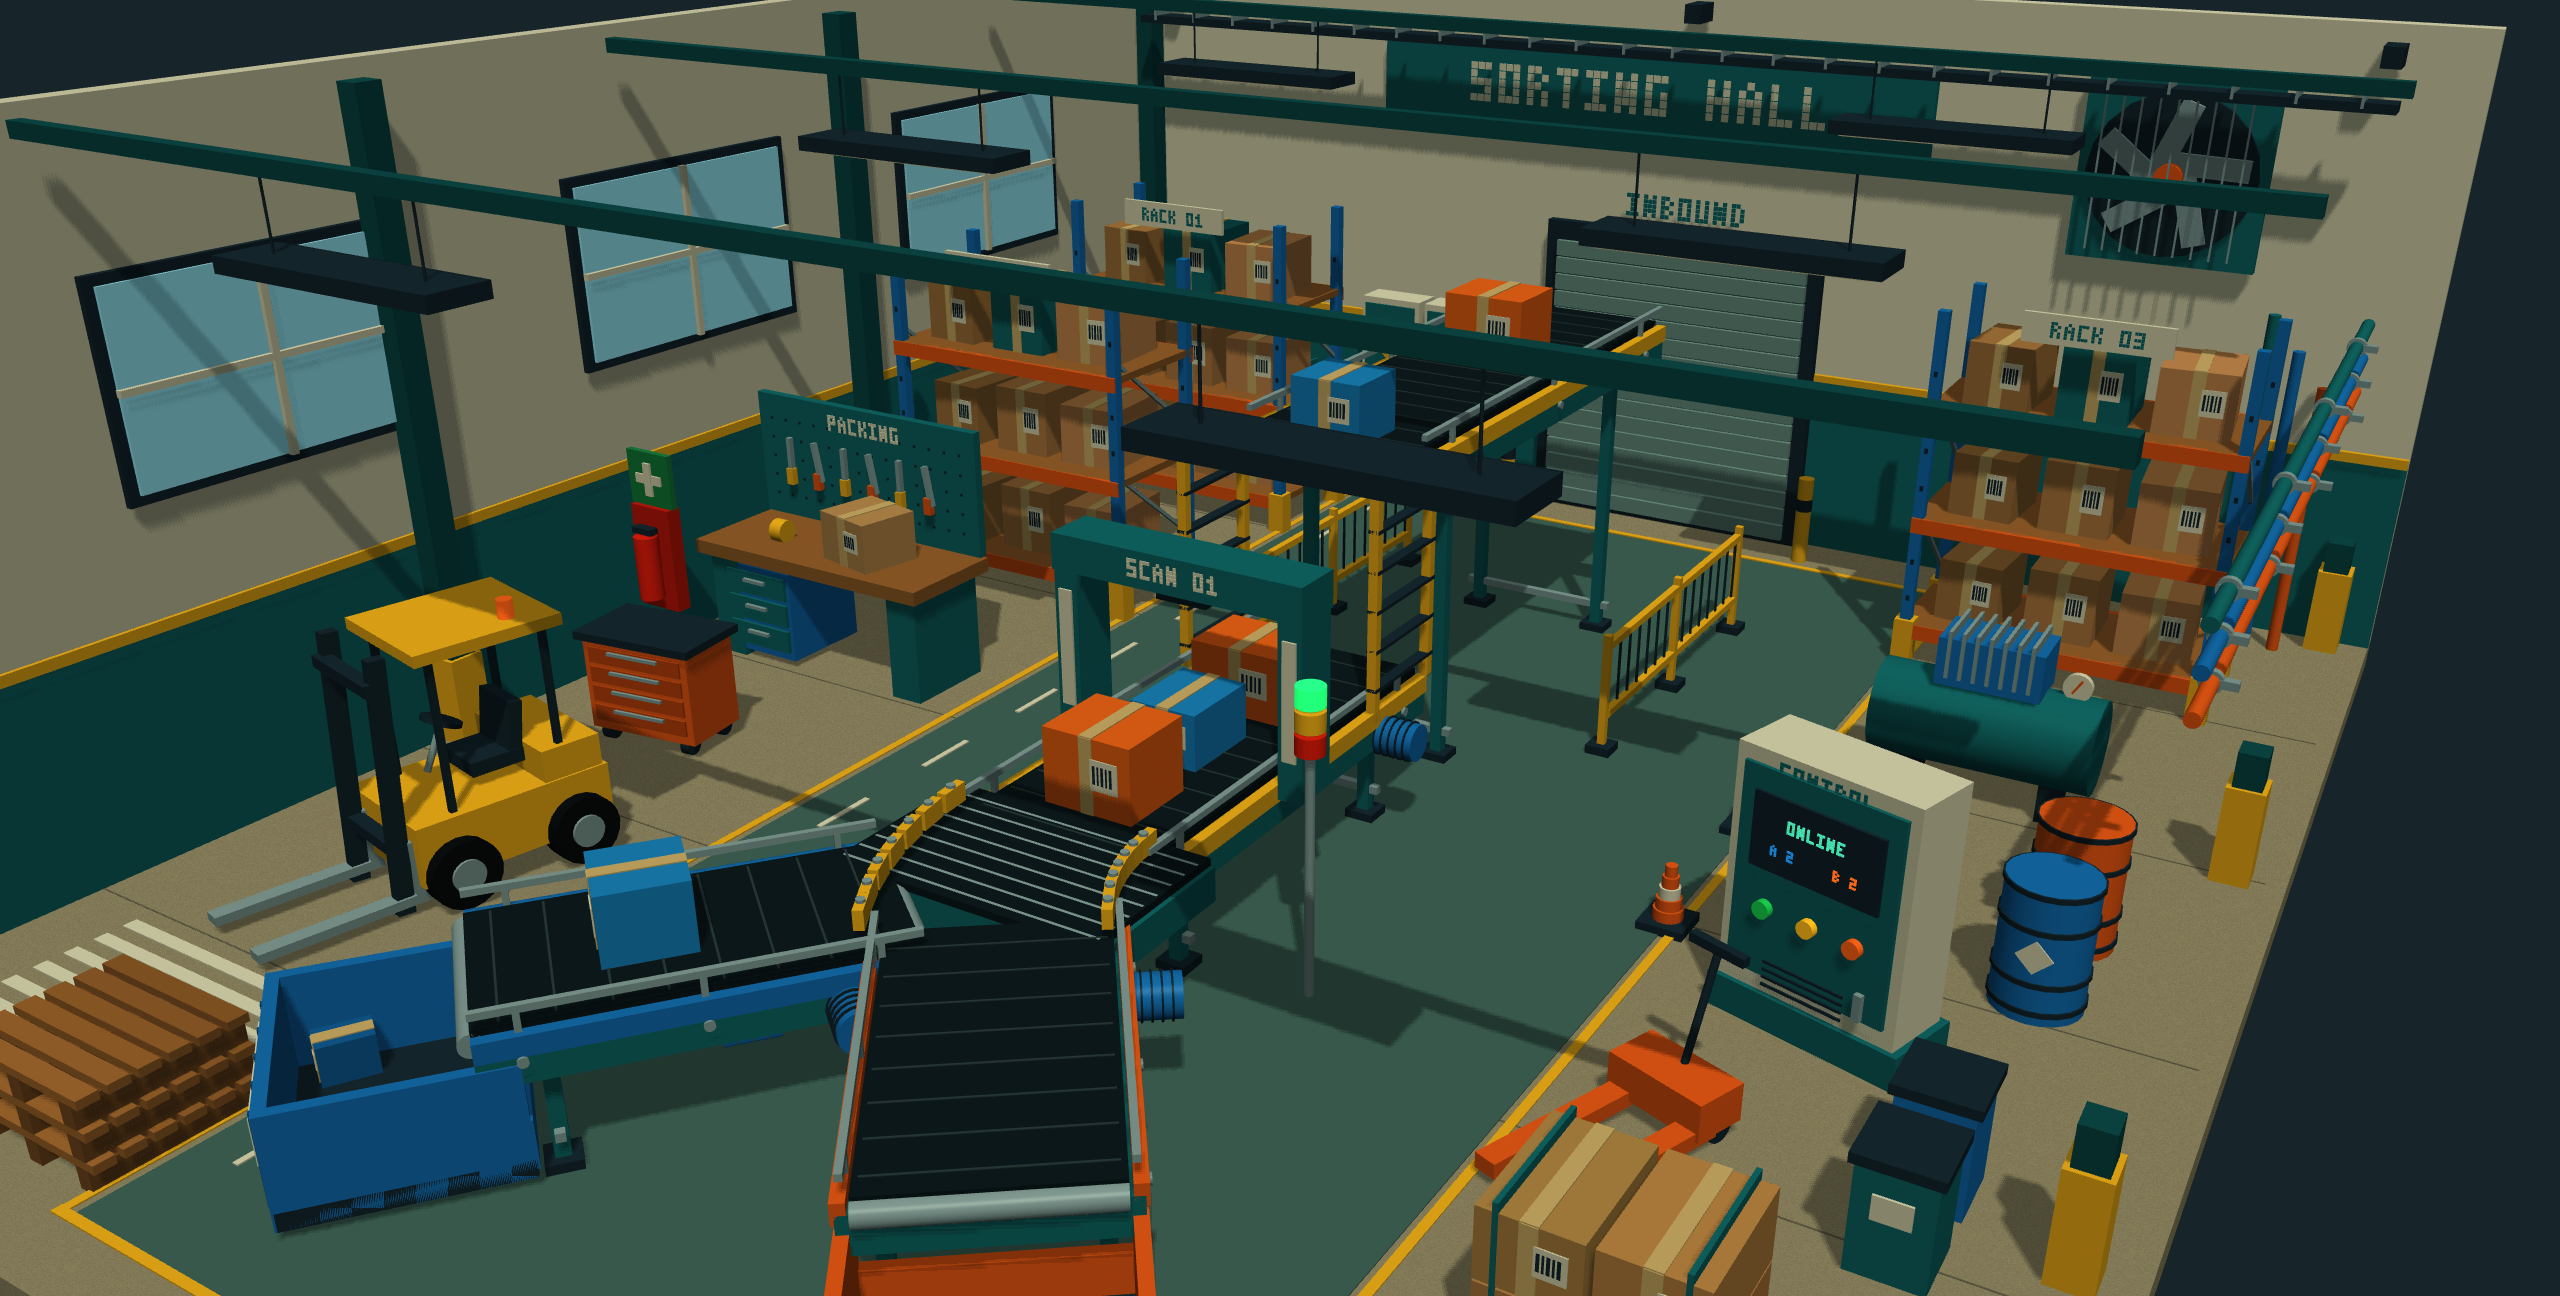
\includegraphics[width=\linewidth]{assets/lights_off_crop.png}\par\small\textbf{B. Point lights off:} ambient and daylight remain.\end{minipage}
\caption{Matched 24 s frames show the effect of the \code{L} toggle. No exposure or color adjustment was applied.}
\end{figure}
\begin{shot}{assets/shadow_detail.png}{Floor and machine detail cropped from the actual rendering. Shadows anchor objects to the floor; repeated markings define the work area.}
\callout{0.60,0.78}{0.18,0.82}{Floor shadow}
\callout{0.66,0.66}{0.78,0.12}{Safety border}
\end{shot}
\subsection{Lighting and surface models}
\textbf{Point lights:} four warm lights at $(\pm4.8,6.75,-6)$ and $(\pm4.8,6.75,5)$ use distance attenuation
\begin{equation}
A(d)=\frac{1}{1+0.025d+0.012d^2}.
\end{equation}
Their combined contribution is $0.36\sum A(d_i)F_i$, where $F_i$ contains diffuse and specular light. Daylight points toward $(10,24,14)$.

\textbf{Shadows:} a 2048 by 2048 light-view depth map stores the nearest surface. The camera pass compares its depth against nine neighboring samples (3 by 3 PCF). Shadow fraction $q=n_{blocked}/9$ reduces daylight by $1-0.78q$. A small depth bias prevents false self-shadows; point lights do not cast shadows.

\textbf{Emission:} $eB$ brightens lamps, scan lines and text. It has no bloom or nearby illumination. \textbf{Floor grain:} $c=\lfloor95(p_x,p_z)\rfloor$, $g=\operatorname{fract}(\sin(c\cdot(12.9898,78.233))43758.5453)$ and $f=0.95+0.10g$ slightly vary floor color. No image texture is loaded.

The shader adds ambient, shadowed daylight, enabled point lights and emission, then applies color rolloff $C_{out}=C_{pre}/(1+0.22C_{pre})$. Output is opaque; there is no gamma-correction stage.
\source{\code{main.cpp}: light uniforms and shadow passes; \code{basic.frag}: \code{shadowAmount()}, floor grain, emission and final color.}
